\documentclass[12pt]{article}

% =========================
% Packages
% =========================
\usepackage[margin=1in]{geometry}
\usepackage{setspace}
\usepackage{booktabs}
\usepackage{longtable}
\usepackage{array}
\usepackage{amsmath}
\usepackage{amssymb}
\usepackage{amsthm}
\usepackage{hyperref}
\usepackage{tikz}
\usetikzlibrary{positioning,arrows.meta}
\usepackage{graphicx}
\usepackage{placeins}

\hypersetup{
  colorlinks=true,
  linkcolor=black,
  urlcolor=blue,
  citecolor=black
}

\setlength{\parskip}{0.6em}
\setlength{\parindent}{0pt}
\setlength{\belowcaptionskip}{10pt}
\onehalfspacing

\newcolumntype{C}[1]{>{\centering\arraybackslash}p{#1}}

% =========================
% Document
% =========================
\begin{document}

\begin{center}
{\LARGE \textbf{The Dickinson Climate Classification: A Taxonomic Thermal-Hydrological Partition of Climate State Space}}\\
\vspace{0.25em}
{\large Caleb Dickinson}
\end{center}

\section*{Abstract}

This paper introduces the Dickinson Climate Classification, a taxonomy that partitions climate state space using evenly spaced thermal metrics and scale-invariant hydrological metrics rather than biological criteria. Unlike widely used frameworks such as the Köppen classification or the UNEP aridity index, which are calibrated to present-day vegetation distributions or land-degradation objectives, the Dickinson system is formulated as a taxonomic division of climates relevant to the persistence of life. Cold-month and warm-month thermal zones are defined using evenly spaced climatological temperature intervals, while moisture regimes are determined exclusively by dimensionless precipitation-to–potential evapotranspiration (P/PET) ratios and precipitation seasonality metrics, ensuring invariance under uniform rescaling of hydrological fluxes. The resulting framework provides a classification applicable across paleoclimates, present-day conditions, extreme future warming scenarios, and hypothetical climate states without requiring recalibration as biological tolerances evolve. This system is particularly suited for identifying emergent climates with no modern analogues and situating Earth’s climates within a broader climate state space.

\section*{Document Status and Scope}

This manuscript presents a formal climate classification framework.
It is not a predictive climate model, attribution study, or impact assessment.
The system is intended as a taxonomic and analytical tool for
comparing climate regimes across paleoclimates, future warming
scenarios, and ecologically relevant climatic states that may never be
realized on Earth, without requiring revision of thresholds or category
definitions. This manuscript is released as a preprint to establish a persistent, citable description of the Dickinson Climate Classification framework, and is distributed under a Creative Commons Attribution–NonCommercial 4.0 International License.

\section*{Data and Implementation Notes}

All illustrative maps were generated using Google Earth Engine
from CHELSA BIOCLIM+ v2.1 1981--2010 climatological normals (Karger et al., 2017; Brun et al., 2022). No new climate model simulations were performed for this work.
The classification logic is deterministic and reproducible.

\section*{Introduction}

The Dickinson Climate Classification differs in both purpose
and structure from widely used systems. The Köppen system (Köppen, 1884) is ecological and biogeographic, with classification thresholds calibrated to the present-day distribution of vegetation and climatic analogues on Earth. The UNEP aridity index (UNEP, 1992) is development-oriented, designed primarily to assess land
degradation and desertification. In contrast, the Dickinson classification is formulated
as a thermodynamic partition of climate state space, independent of
biological distributions and socioeconomic objectives.

Let $\mathcal{C}_{\mathrm{life}}$ denote the subset of climate state space thermodynamically compatible with the persistence of life.
Let $T_{\min}^{\mathrm{life,low}}$ and
$T_{\min}^{\mathrm{life,high}}$ denote the lower and upper bounds,
respectively, of climatological coldest-month mean temperature compatible
with life, and let $T_{\max}^{\mathrm{life,low}}$ and
$T_{\max}^{\mathrm{life,high}}$ denote the corresponding bounds for
climatological warmest-month mean temperature.

The Dickinson classification is defined only for climates satisfying
\[
T_{\min}^{\mathrm{life,low}} \le T_{\min,\mathrm{mean}}
\le T_{\min}^{\mathrm{life,high}}, \qquad
T_{\max}^{\mathrm{life,low}} \le T_{\max,\mathrm{mean}}
\le T_{\max}^{\mathrm{life,high}},
\]
with the physical constraint $T_{\min,\mathrm{mean}} \le T_{\max,\mathrm{mean}}$.
These thermodynamic life bounds are not estimated in this work.

\paragraph{Note.} Microbial activity has been documented in snow at the geographic
South Pole (Carpenter et al., 2000), an environment whose
climatological monthly mean temperatures correspond to the
YY (superarctic with frigid summer) thermal regime in the
Dickinson classification. This observation demonstrates that
the coldest thermal regime defined in the system occurs within
the domain of climates known to support microbial life.

Biological tolerances are not fixed: they shift over evolutionary time as
lineages diverge from common ancestors and adapt to changing environmental
conditions. Systems calibrated to contemporary species distributions
therefore embed historical contingency and lose validity when applied to
deep-time climates or extreme future scenarios. Thus, classification thresholds in the Dickinson system are independent of the present-day distribution limits of biological taxa.

Millimeter-based precipitation thresholds do not represent equivalent hydrological constraints across climates with different thermal regimes: a fixed precipitation total implies fundamentally different surface water availability in cold versus hot environments due to large differences in evaporative demand. For this reason, aridity regimes in the Dickinson system are defined exclusively using dimensionless ratios of hydrological quantities. No aridity boundary is specified in terms of absolute precipitation totals, absolute evapotranspiration totals, or fixed millimeter thresholds. Instead, aridity classification depends solely on relative water balance and is therefore invariant under uniform rescaling of hydrological fluxes.

The Dickinson classification is intended as a partition of continuous
climate space rather than as a definition of habitability limits. It does
not attempt to identify the absolute bounds of life. Consequently, hypothetical thermophile-dominated regimes with
$T_{\max,\mathrm{mean}} = 55^\circ\mathrm{C}$ versus $80^\circ\mathrm{C}$, for example, may be
assigned to the same category. This design choice preserves classification
stability across paleoclimatic variability, evolutionary adaptation, and
extreme future warming scenarios, without requiring revision in response
to newly discovered extremophiles or altered biological tolerances.

Under strong anthropogenic warming, Earth is expected to enter climatic regimes with no present-day analogues, characterized by combinations of thermal and hydrological conditions not historically observed. Classification systems calibrated to modern Earth climate distributions perform well for climates resembling those present at the time of their formulation, but can yield misleading classifications under novel conditions. For example, a hypothetical location with constant rainfall and identical monthly mean temperatures to present-day Phoenix, Arizona would be classified as humid subtropical (Cfa) under Köppen, despite occupying a far more thermodynamically extreme regime than locations such as Tokyo or Atlanta. The Dickinson Climate Classification is designed to address this limitation, providing a framework for tracking climate regime transitions under strong warming, identifying emergent climates with no modern analogues, and comparing paleoclimatic and future states within a single classification scheme.

Additionally, the structure of this system permits higher categorical resolution than most legacy climate classification frameworks. Because thermal and hydrological categories are defined using evenly spaced physical metrics rather than empirically tuned ecological thresholds, the classification can be applied at fine spatial scales wherever reliable climatological normals are available. This property makes the framework well suited to resolving sharp climatic gradients, topographic microclimates, and human-relevant thermal regimes without requiring additional calibration or region-specific adjustment.

The system is defined only over the subset of climate space in which the
persistence of life is physically possible. Outside this domain, the classification is not
meaningful and no interpretation is implied.

\begin{table}[htbp]
\centering
\caption{Conceptual comparison of major climate classification frameworks, including the Dickinson system, the Köppen classification, the Holdridge bioclimatic life-zone scheme (Holdridge, 1947), and the UNEP aridity index.
}
\renewcommand{\arraystretch}{1.35}
\begin{tabular}{|C{3.1cm}|C{3.8cm}|C{4.1cm}|C{3.8cm}|}
\hline
\textbf{Framework} &
\textbf{Primary variables} &
\textbf{Calibration basis} &
\textbf{Applicability} \\
\hline
Köppen (1884) &
Temperature and precipitation thresholds &
Observed vegetation distributions &
Present-day Earth climates; limited extrapolation \\
\hline
Holdridge (1947) &
Biotemperature, precipitation, $P/PET$ &
Plant physiological response &
Ecological zoning; biologically contingent \\
\hline
UNEP (1992) &
Annual $P/PET$ &
Land degradation and desertification risk &
Development-oriented; aridity only \\
\hline
Dickinson\par\vspace{0.2\baselineskip}(this work) &
Cold-month $T_{\min}$, warm-month $T_{\max}$, $P/PET$, seasonality &
Thermodynamic partition of climate state space &
Paleoclimates, future climates, hypothetical states \\
\hline
\end{tabular}
\end{table}

% ============================================================
\section{Thermal Metrics and Cold-Month Thermal Zones}

Thermal classification in the Dickinson system is based on climatological
monthly mean near-surface air temperatures, computed over a standard
30-year normal period. For each location, the coldest-month mean
temperature is taken as the minimum of the twelve climatological monthly
means, while the warmest-month mean temperature is taken as the maximum.

The cold-month thermal intervals are defined in uniform increments of 10 °C, with 5 °C resolution used for all but one warm-month category; the \textit{hyperthermal summer} category retains 10 °C spacing. These intervals correspond to simple fractional subdivisions of the 100 °C temperature span between the freezing and boiling points of water at standard pressure. This choice provides a reproducible reference scale without implying special physical thresholds at category boundaries.

The choice of thermal binning reflects a balance between physical
interpretability and classification stability, with asymmetric resolution
applied to cold- and warm-month metrics. Cold-month thermal zones are
defined using uniform 10~$^\circ$C intervals, as winter temperature
primarily acts as a threshold constraint on surface processes, cryospheric
state, and large-scale habitability. Differences smaller than this scale do
not typically distinguish fundamentally different winter regimes at the
global level, while coarser intervals would collapse thermodynamically
distinct cold states.

By contrast, the warm-month thermal axis is partitioned at higher resolution, using 5~$^\circ$C intervals when a given temperature occurs as a warmest-month mean rather than as a coldest-month mean, across the range of monthly mean temperatures from $\geq 0$ to $<40~^\circ$C. This reflects the continuous and highly sensitive influence of summer warmth on surface energy balance, evapotranspiration, and heat stress. Accordingly, cold-month thermal classes C, B, A, and Z—defined by their coldest-month means—are each subdivided into paired warm-month categories when their warmest-month means fall within these same numerical temperature intervals (e.g., C into c1 and c2, B into b1 and b2, with analogous subdivisions for A and Z).

This asymmetric treatment follows long-standing precedent in climate classification. In the Köppen system, for example, the temperature spacing between winter-regime isotherms is substantially broader than that separating summer heat regimes (Köppen, 1884). The combined use of uniform 10~$^\circ$C cold-month bins and finer warm-month subdivisions therefore produces a transparent, scale-consistent partition of climate space that remains robust across paleoclimates, projected future warming scenarios, and hypothetical climate states.

Cold-month thermal zones are assigned using the climatological
coldest-month mean temperature ($T_{\min,\mathrm{mean}}$), which provides a measure of winter thermal constraint that is insensitive to short-
duration extremes. The resulting cold-month thermal zones span the full
range of physically plausible climates, from extreme cold environments to
hypothetical hyperthermal regimes that may occur under deep-time or future
boundary conditions.

Based on $T_{\min,\mathrm{mean}}$, climates are assigned to one of the
following cold-month thermal zones:
\[
\begin{array}{ll}
\text{Hypercaneal (H)}        &
50^\circ\mathrm{C} \le T_{\min,\mathrm{mean}}
\le T_{\min}^{\mathrm{life,high}} \\
\text{Uninhabitable (X)}      & 40 \le T_{\min,\mathrm{mean}} < 50^\circ\mathrm{C} \\
\text{Hyperequatorial (Z)}    & 30 \le T_{\min,\mathrm{mean}} < 40^\circ\mathrm{C} \\
\text{Equatorial (A)}         & 20 \le T_{\min,\mathrm{mean}} < 30^\circ\mathrm{C} \\
\text{Tropical (B)}           & 10 \le T_{\min,\mathrm{mean}} < 20^\circ\mathrm{C} \\
\text{Subtropical (C)}        & 0 \le T_{\min,\mathrm{mean}} < 10^\circ\mathrm{C} \\
\text{Temperate (D)}          & -10 \le T_{\min,\mathrm{mean}} < 0^\circ\mathrm{C} \\
\text{Continental (E)}        & -20 \le T_{\min,\mathrm{mean}} < -10^\circ\mathrm{C} \\
\text{Subarctic (F)}          & -30 \le T_{\min,\mathrm{mean}} < -20^\circ\mathrm{C} \\
\text{Arctic (G)}             & -40 \le T_{\min,\mathrm{mean}} < -30^\circ\mathrm{C} \\
\text{Superarctic (Y)}        &
T_{\min}^{\mathrm{life,low}}
\le T_{\min,\mathrm{mean}} < -40^\circ\mathrm{C}
\end{array}
\]

These thresholds are evenly spaced in temperature and are intended to
represent thermodynamic regimes rather than ecological boundaries. As a
result, the classification remains applicable across paleoclimates,
projected future climates, and hypothetical climate states without
requiring recalibration to present-day biological distributions.

\paragraph{Note on the term ``Uninhabitable''.}
\emph{Uninhabitable} denotes climates for which the coldest-month
climatological mean temperature satisfies
$40^\circ\mathrm{C} \le T_{\min,\mathrm{mean}} < 50^\circ\mathrm{C}$, implying
that all monthly means exceed the core body temperature of humans and other
large mammals. The term is thermodynamic in scope and does not preclude
habitation by organisms with substantially different size, physiology, or
thermal regulation strategies than large mammals, nor technologically
mediated habitation.

\paragraph{Note on hypercanes.}
The term \emph{hypercaneal} is used here strictly as a thermal descriptor for extremely hot climatological monthly mean temperatures. Hypercaneal cold-month and/or warm-month thermal zones should be understood as a \emph{necessary but not sufficient} condition for the formation of hypercane vortices (Emanuel, 1988). Hypercane development also depends on additional dynamical and oceanic factors that are not represented in a monthly-mean thermal
classification. Accordingly, classification as hypercaneal does not imply the existence, frequency, or persistence of hypercanes.

\clearpage

\begin{figure}[htbp]
\centering
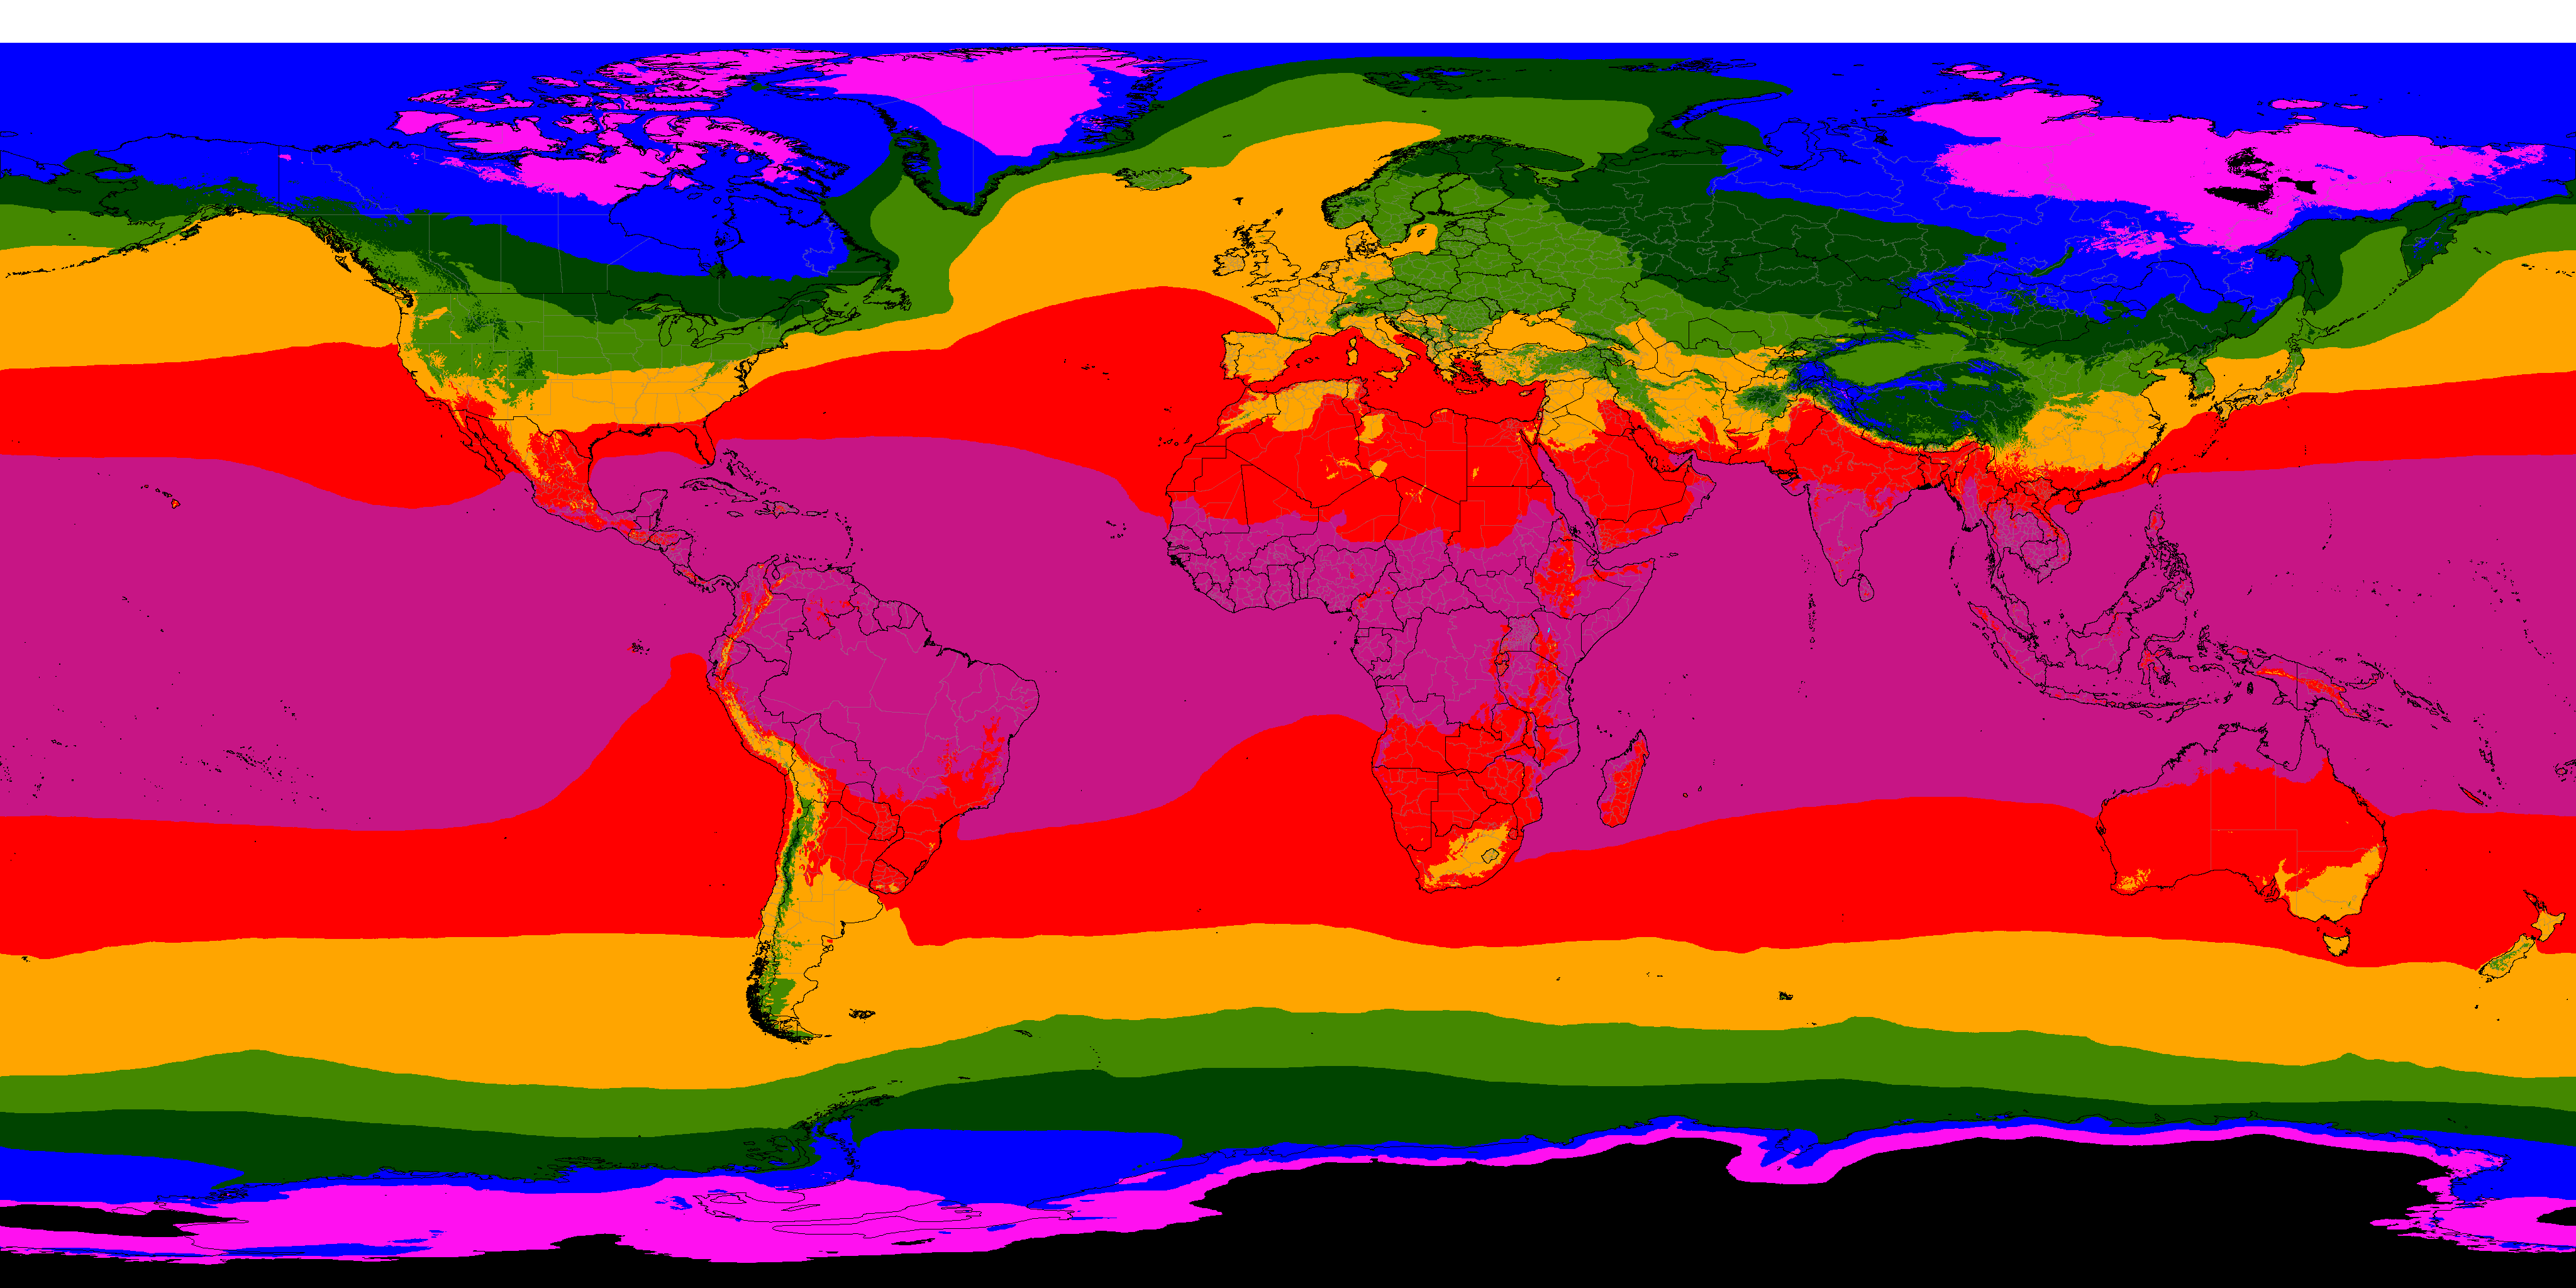
\includegraphics[width=\textwidth]{global_cold_month_1981-2010.png}
\label{fig:global_cold_month}
\end{figure}

\begin{figure}[htbp]
\centering
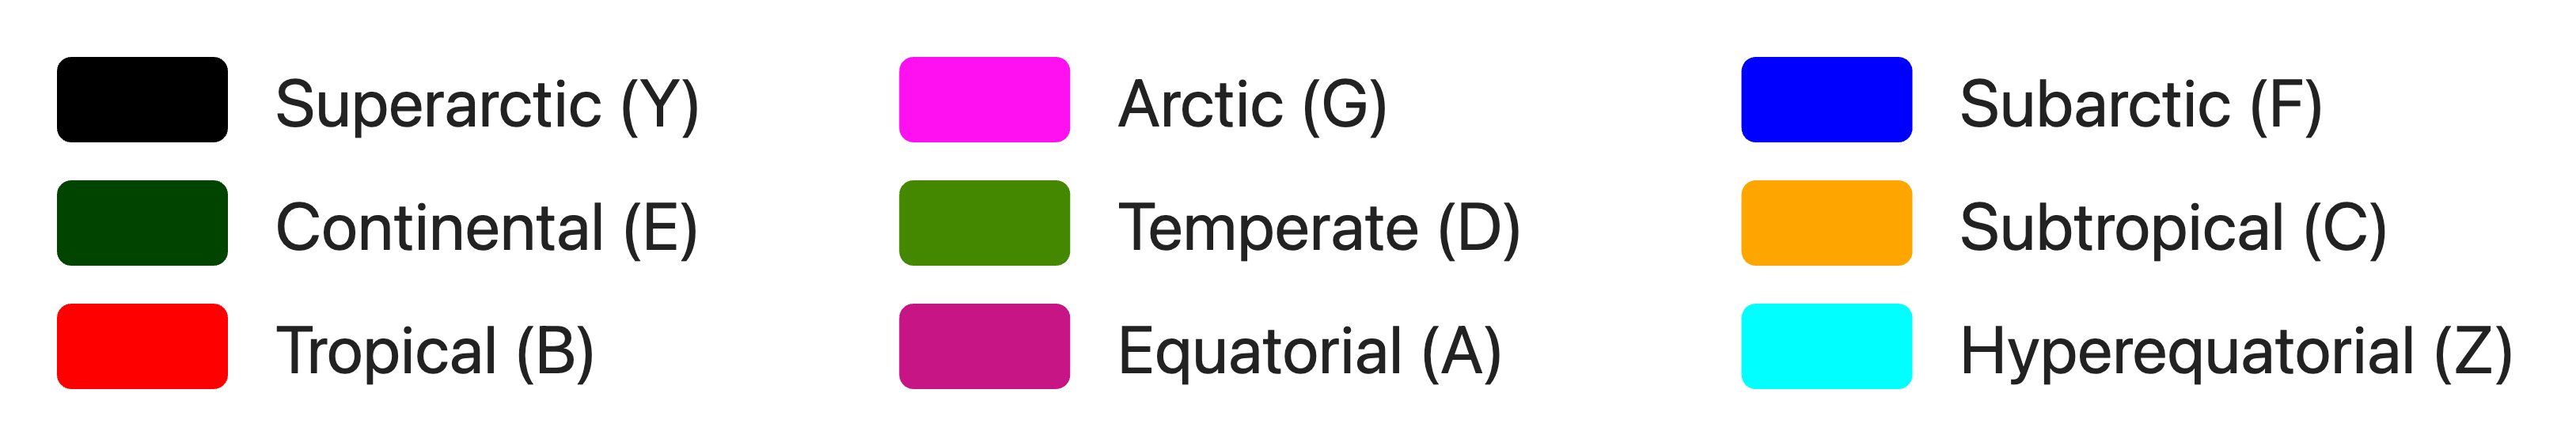
\includegraphics[width=\textwidth]{cold_month_legend.png}
\caption{
Global distribution of cold-month thermal zones under the
Dickinson Climate Classification, based on 1981--2010 climatological normals.
Data were processed and plotted in Google Earth Engine (GEE) using
CHELSA BIOCLIM+ v2.1 1981--2010 temperature fields (Karger et al., 2017; Brun et al., 2022).
}
\label{fig:cold_month_legend}
\end{figure}

\clearpage

% ============================================================
\section{Warm-Month Thermal Zones}

In addition to cold-season thermal constraints, the Dickinson
classification characterizes the intensity of the warm season using the
climatological warmest-month mean near-surface air temperature
($T_{\max,\mathrm{mean}}$). This metric provides a measure of summer
thermal conditions that reflects seasonal energy balance rather than
short-lived extreme events.

Warm-month thermal zones are assigned based on $T_{\max,\mathrm{mean}}$ and
are intended to distinguish climates with similar winter conditions but
substantially different summer heat regimes. The resulting categories span
the full range of plausible summer thermal environments, from persistently
cold summers to extreme hyperthermal regimes that may occur under deep-time
or future warming scenarios.

Based on the warmest-month mean temperature, climates are assigned to one
of the following warm-month thermal zones:
\[
\begin{array}{ll}
\text{Hypercaneal Summer (H)} &
50^\circ\mathrm{C} \le T_{\max,\mathrm{mean}}
\le T_{\max}^{\mathrm{life,high}} \\
\text{Hyperthermal Summer (X)}     & 40 \le T_{\max,\mathrm{mean}} < 50^\circ\mathrm{C} \\
\text{Scorching Summer (z2)}       & 35 \le T_{\max,\mathrm{mean}} < 40^\circ\mathrm{C} \\
\text{Very Hot Summer (z1)}        & 30 \le T_{\max,\mathrm{mean}} < 35^\circ\mathrm{C} \\
\text{Hot Summer (a2)}             & 25 \le T_{\max,\mathrm{mean}} < 30^\circ\mathrm{C} \\
\text{Warm Summer (a1)}            & 20 \le T_{\max,\mathrm{mean}} < 25^\circ\mathrm{C} \\
\text{Cool Summer (b2)}            & 15 \le T_{\max,\mathrm{mean}} < 20^\circ\mathrm{C} \\
\text{Cold Summer (b1)}            & 10 \le T_{\max,\mathrm{mean}} < 15^\circ\mathrm{C} \\
\text{Very Cold Summer (c2)}       & 5 \le T_{\max,\mathrm{mean}} < 10^\circ\mathrm{C} \\
\text{Freezing Summer (c1)}        & 0 \le T_{\max,\mathrm{mean}} < 5^\circ\mathrm{C} \\
\text{Frigid Summer (Y)} &
T_{\max}^{\mathrm{life,low}}
\le T_{\max,\mathrm{mean}} < 0^\circ\mathrm{C}
\end{array}
\]

As with the cold-month thermal zones, warm-month thresholds are evenly
spaced in temperature and are intended to represent thermodynamic regimes
rather than biological or impact-based categories. This approach ensures
consistency across paleoclimates, present-day climates, and projected
future warming scenarios without reliance on species-specific tolerance
limits or human comfort thresholds.

\clearpage

\begin{figure}[htbp]
\centering
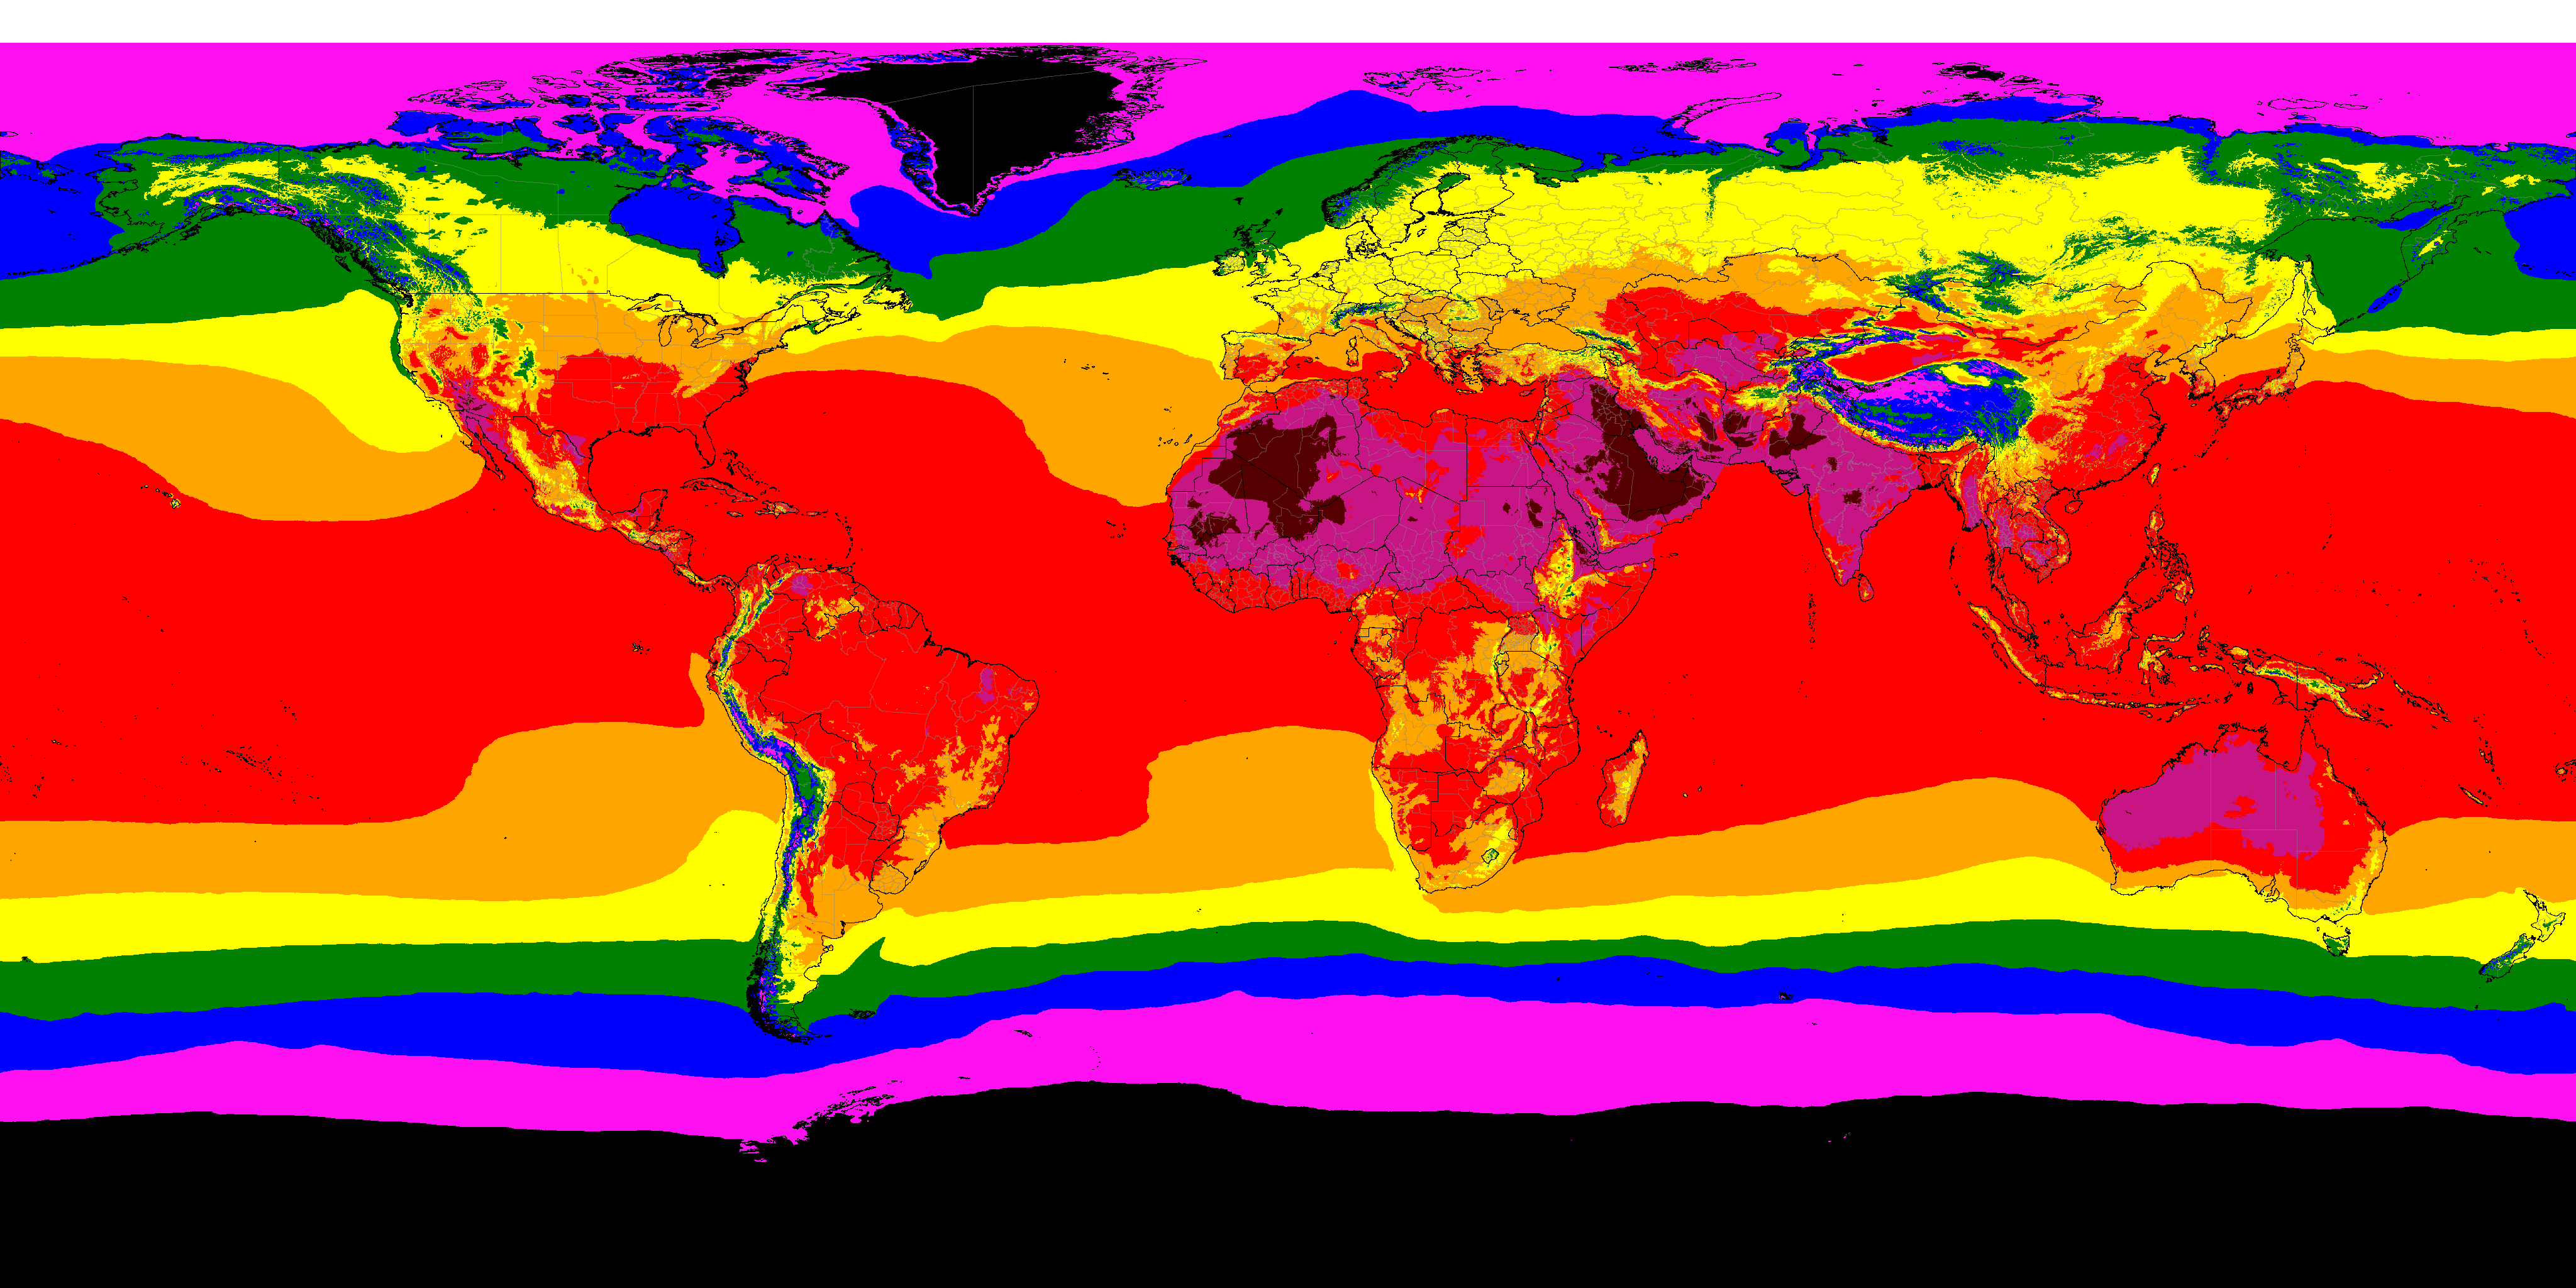
\includegraphics[width=\textwidth]{global_warm_month_1981-2010.png}
\label{fig:global_warm_month}
\end{figure}

\begin{figure}[htbp]
\centering
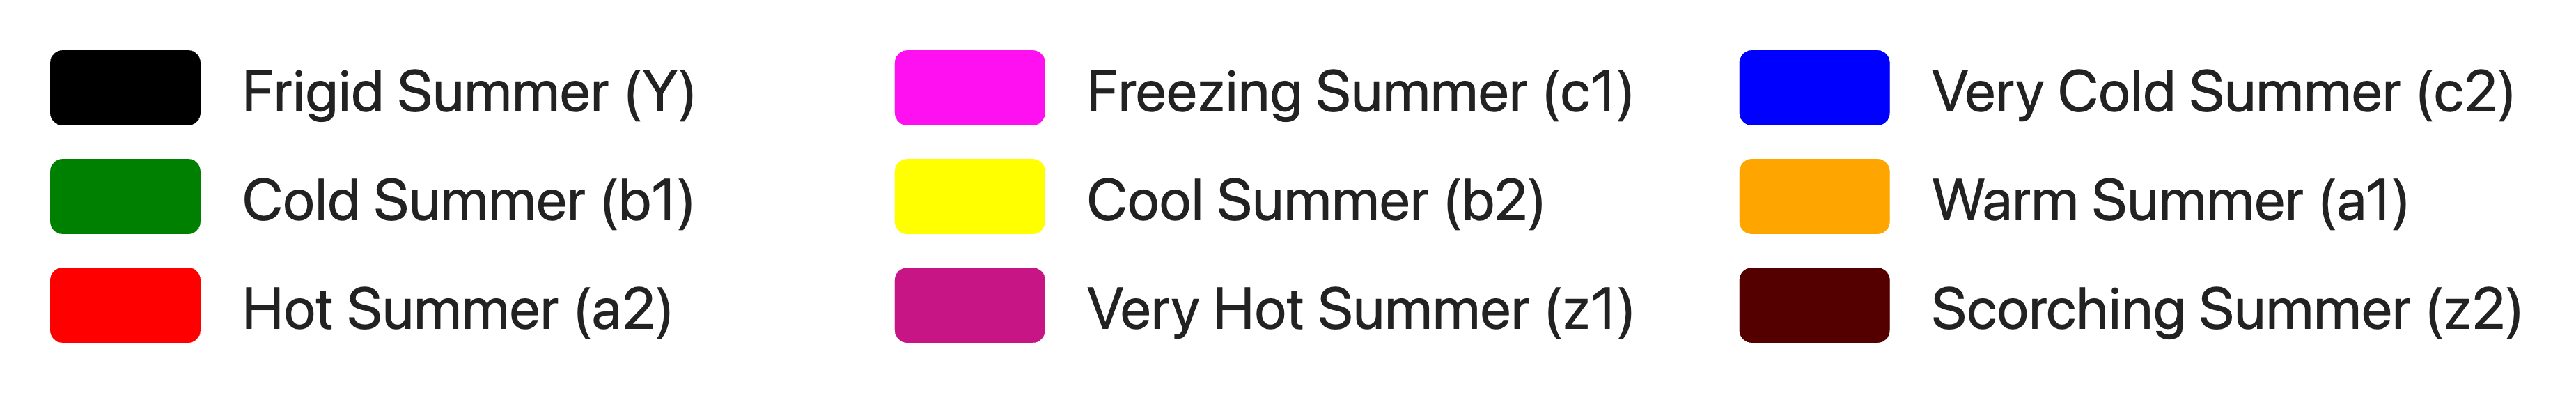
\includegraphics[width=\textwidth]{warm_month_legend.png}
\caption{
Global distribution of warm-month thermal zones under the
Dickinson Climate Classification, based on 1981--2010 climatological normals.
Data were processed and plotted in Google Earth Engine (GEE) using
CHELSA BIOCLIM+ v2.1 1981--2010 temperature fields (Karger et al., 2017; Brun et al., 2022).
}
\label{fig:warm_month_legend}
\end{figure}
\FloatBarrier

\clearpage

% ============================================================
\section{Aridity Relevance and Aridity Regimes}

Previous climate classification frameworks have implicitly recognized that aridity diagnostics are meaningful only within a limited thermal domain. In the Köppen system (Köppen, 1884), aridity-based categories are restricted to climates whose climatological warmest-month mean temperature exceeds 10 °C, thereby excluding cold-summer and polar regimes in which surface processes are primarily energy-limited rather than moisture-limited. Similarly, the United Nations Environment Programme (UNEP) aridity framework (UNEP, 1992) distinguishes “cold” regions (annual PET $< 400\,\mathrm{mm}$) from aridity regimes defined by P/PET ratios, acknowledging that water-balance diagnostics lose interpretive value where evaporative demand is minimal.

Moisture regime classification in the Dickinson system is applied only to
climates in which aridity meaningfully structures surface–atmosphere
interactions. Specifically, aridity diagnostics are evaluated only at
locations where the warmest-month mean temperature
($T_{\max,\mathrm{mean}}$) is at least $15^\circ\mathrm{C}$ and the
coldest-month mean temperature ($T_{\min,\mathrm{mean}}$) is at
least $-30^\circ\mathrm{C}$. Together, these constraints define a conservative thermal envelope within which aridity diagnostics exert first-order influence on climate differentiation. Outside this envelope, climates are classified exclusively on thermal grounds.
Consequently, polar, subarctic, alpine, and other climates, such as cold-summer oceanic regimes analogous to
K\"oppen's subpolar oceanic climates, receive no aridity
classification within the Dickinson framework.

At locations that do not satisfy these thermal screening criteria, no
aridity regime is assigned and the moisture classification is not evaluated within the Dickinson framework.
Within this cold thermal regime, aridity diagnostics are not evaluated
over either land or ocean. Outside the regime, aridity classification is
applied only to terrestrial climates.

For climates meeting the aridity relevance criteria, moisture regimes are
defined using the annual aridity index
\[
AI = \frac{P_{\text{ann}}}{PET_{\text{ann}}},
\]
where annual precipitation is computed as the sum of monthly precipitation
totals and where PET denotes annual potential evapotranspiration. All aridity regimes are defined using this dimensionless ratio, ensuring invariance under uniform rescaling of hydrological fluxes.

Based on the annual aridity index, climates are assigned to one of four
baseline aridity regimes in the Dickinson classification:
\[
\begin{array}{ll}
\text{Humid (h)}        & AI \ge 0.75 \\
\text{Semihumid (g)}    & 0.50 \le AI < 0.75 \\
\text{Semiarid (s)}     & 0.25 \le AI < 0.50 \\
\text{Arid (d)}  & AI < 0.25
\end{array}
\]

For comparison, the United Nations Environment Programme (UNEP) aridity
index defines the following regimes:
\[
\begin{array}{ll}
\text{Humid}            & AI \ge 0.65 \\
\text{Dry subhumid}     & 0.50 \le AI < 0.65 \\
\text{Semi-arid}        & 0.20 \le AI < 0.50 \\
\text{Arid}             & 0.05 \le AI < 0.20 \\
\text{Hyper-arid}       & AI < 0.05
\end{array}
\]

The Dickinson aridity thresholds are modified from the UNEP
scheme to provide a more uniform partition of climate space. UNEP's \textit{hyper-arid} and \textit{arid} are incorporated into a single arid category, and each range is
repartitioned to produce evenly spaced, analytically comparable moisture
regimes. This design choice emphasizes thermodynamic consistency and
stability across paleoclimates and future warming scenarios rather than
land-degradation or development-focused classification objectives.

% ============================================================
\section{Seasonality Diagnostics and Aridity Overrides}

In addition to annual water balance, the Dickinson classification
incorporates precipitation seasonality diagnostics to distinguish climates
with similar aridity indices but fundamentally different seasonal
structures. Two complementary diagnostics are used: a high-sun
precipitation fraction and a rolling six-month precipitation dominance
metric.

The high-sun precipitation fraction ($HS$) quantifies the proportion of
annual precipitation occurring during the six highest-insolation months; April-September in the Northern Hemisphere astronomical extratropics, and October-March in the Southern Hemisphere astronomical extratropics. Annual precipitation during this period ($P_{\text{hs}}$) is divided by
total annual precipitation ($P_{\text{ann}}$) to yield
\[
HS = \frac{P_{\text{hs}}}{P_{\text{ann}}}.
\]
This diagnostic captures hemispherically asymmetric seasonal regimes, particularly extratropical climates characterized by dry summers and wet winters.

To identify strongly concentrated wet seasons independent of calendar
alignment, a rolling six-month precipitation dominance metric is also
computed. For each possible six-month window, cumulative precipitation is
evaluated, and the maximum total ($P6$) is normalized by annual
precipitation to yield
\[
P6_{\text{ratio}} = \frac{P6}{P_{\text{ann}}}.
\]
This metric detects monsoonal regimes in which the majority of annual
precipitation occurs within a contiguous portion of the year, regardless
of its seasonal timing.

These seasonality diagnostics are applied as overrides to the baseline
aridity regimes to distinguish Mediterranean and monsoonal climates.

\emph{Mediterranean} climates are identified as non-arid regimes
($AI \ge 0.25$) exhibiting strong winter precipitation dominance in the
astronomical extratropics ($HS < 0.4$).

\emph{Monsoon} climates are identified using the rolling six-month precipitation
dominance metric. Climates in which at least 80\% of annual precipitation
occurs within any consecutive six-month period
($P6_{\text{ratio}} \ge 0.8$) are classified as monsoonal, excluding climates
already classified as arid or Mediterranean.

Climates meeting the monsoon criterion are classified as \emph{Semiarid Monsoon} when $AI < 0.50$, to distinguish them from monsoon climates with semihumid or humid aridity indices.

Finally, a temperate rainforest override is applied to prevent
Mediterranean classification in climates that remain persistently moist
throughout the year. For climates initially identified as Mediterranean,
the minimum monthly precipitation ($P_{\text{driest}}$) is compared to
annual potential evapotranspiration. If
\[
P_{\text{driest}} \ge \frac{PET_{\text{ann}}}{24},
\]
the climate is reclassified as humid. This criterion corresponds to a
minimum monthly precipitation of at least 50\% of mean monthly PET.

\begin{figure}[htp]
\centering
\resizebox{\textwidth}{!}{%
\begin{tikzpicture}[
  node distance=12mm and 16mm,
  decision/.style={
    rectangle, draw, rounded corners,
    align=center, font=\small,
    minimum width=4.8cm, minimum height=9mm
  },
  outcome/.style={
    rectangle, draw,
    align=center, font=\small,
    fill=gray!10,
    minimum width=4.8cm, minimum height=9mm
  },
  arrow/.style={->, thick}
]

% =====================================================
% START
% =====================================================

\node[decision] (relevance)
{$T_{\max,\mathrm{mean}} \ge 15\,^\circ\mathrm{C}$\\
$\text{and } T_{\min,\mathrm{mean}} \ge -30\,^\circ\mathrm{C}$?}

\node[outcome, left=of relevance] (polar)
{aridity not evaluated};

\draw[arrow] (relevance) -- node[above,font=\small]{No} (polar);

% =====================================================
% ARID CHECK
% =====================================================

\node[decision, below=of relevance] (aridcheck)
{$\dfrac{P_{\mathrm{ann}}}{PET_{\mathrm{ann}}} < 0.25$?};

\node[outcome, left=of aridcheck] (arid)
{Arid (d)};

\draw[arrow] (relevance) -- node[left,font=\small]{Yes} (aridcheck);
\draw[arrow] (aridcheck) -- node[above,font=\small]{Yes} (arid);

% =====================================================
% MEDITERRANEAN CHECK
% =====================================================

\node[decision, below=of aridcheck] (medcheck)
{$|\phi| > \varepsilon$\\
\text{and} $HS < 0.4$?};

\draw[arrow] (aridcheck) -- node[left,font=\small]{No} (medcheck);

\node[decision, right=of medcheck] (medoverride)
{$P_{\text{driest}} < \dfrac{PET_{\text{ann}}}{24}$?};

\node[outcome, below=of medoverride] (humid)
{Humid (h)};

\node[outcome, above=of medoverride] (med)
{Mediterranean (m)};

\draw[arrow] (medcheck) -- node[above,font=\small]{Yes} (medoverride);
\draw[arrow] (medoverride) -- node[left,font=\small]{No} (humid);
\draw[arrow] (medoverride) -- node[left,font=\small]{Yes} (med);

% =====================================================
% MONSOON CHECK
% =====================================================

\node[decision, below=of medcheck] (monsooncheck)
{$P6_{ratio} \ge 0.8$?};

\draw[arrow] (medcheck) -- node[left,font=\small]{No} (monsooncheck);

% --- Split by dryness if monsoon-dominant ---

\node[decision, left=of monsooncheck] (monsoonsplit)
{$\dfrac{P_{\mathrm{ann}}}{PET_{\mathrm{ann}}} < 0.50$?};

\draw[arrow] (monsooncheck) -- node[above,font=\small]{Yes} (monsoonsplit);

% --- Outcomes ---

\node[outcome, above=of monsoonsplit] (semimons)
{Semiarid Monsoon (v)};

\node[outcome, below=of monsoonsplit] (monsoon)
{Monsoon (w)};

\draw[arrow] (monsoonsplit) -- node[left,font=\small]{Yes} (semimons);
\draw[arrow] (monsoonsplit) -- node[left,font=\small]{No} (monsoon);

% =====================================================
% HUMIDITY SPLIT
% =====================================================

\node[decision, below=of monsooncheck] (semiaridcheck)
{$\dfrac{P_{\mathrm{ann}}}{PET_{\mathrm{ann}}} < 0.50$?};

\node[outcome, below=of semiaridcheck] (semiarid)
{Semiarid (s)};

\draw[arrow] (monsooncheck) -- node[left,font=\small]{No} (semiaridcheck);
\draw[arrow] (semiaridcheck) -- node[left,font=\small]{Yes} (semiarid);

\node[decision, right=of semiaridcheck] (semihumidcheck)
{$\dfrac{P_{\mathrm{ann}}}{PET_{\mathrm{ann}}} < 0.75$?};

\draw[arrow] (semiaridcheck) -- node[above,font=\small]{No} (semihumidcheck);

\node[outcome, below=of semihumidcheck] (semihumid)
{Semihumid (g)};

% NOTE: Humid (H) node already exists elsewhere
\draw[arrow] (semihumidcheck) -- node[left,font=\small]{Yes} (semihumid);
\draw[arrow] (semihumidcheck) -- node[left,font=\small]{No} (humid);

\end{tikzpicture}
}

\caption{
Decision tree for assigning aridity regimes in the Dickinson
classification.\\\\
\textbf{Note:} $\phi$ denotes geographic latitude in degrees.
$\varepsilon$ denotes the Earth’s axial tilt (obliquity), defined as the
instantaneous angle between the Earth’s rotational axis and the normal
to its orbital plane. For present-day Earth, $\varepsilon \approx 23.44^\circ$,
but $\varepsilon$ is treated here as a physical parameter rather than a fixed
constant, allowing for secular variation over geological timescales.
In this context, extratropical locations are defined as latitudes poleward
of the astronomical tropics.
Mediterranean seasonality is evaluated only at such locations.
}
\end{figure}

\begin{figure}[htbp]
\centering
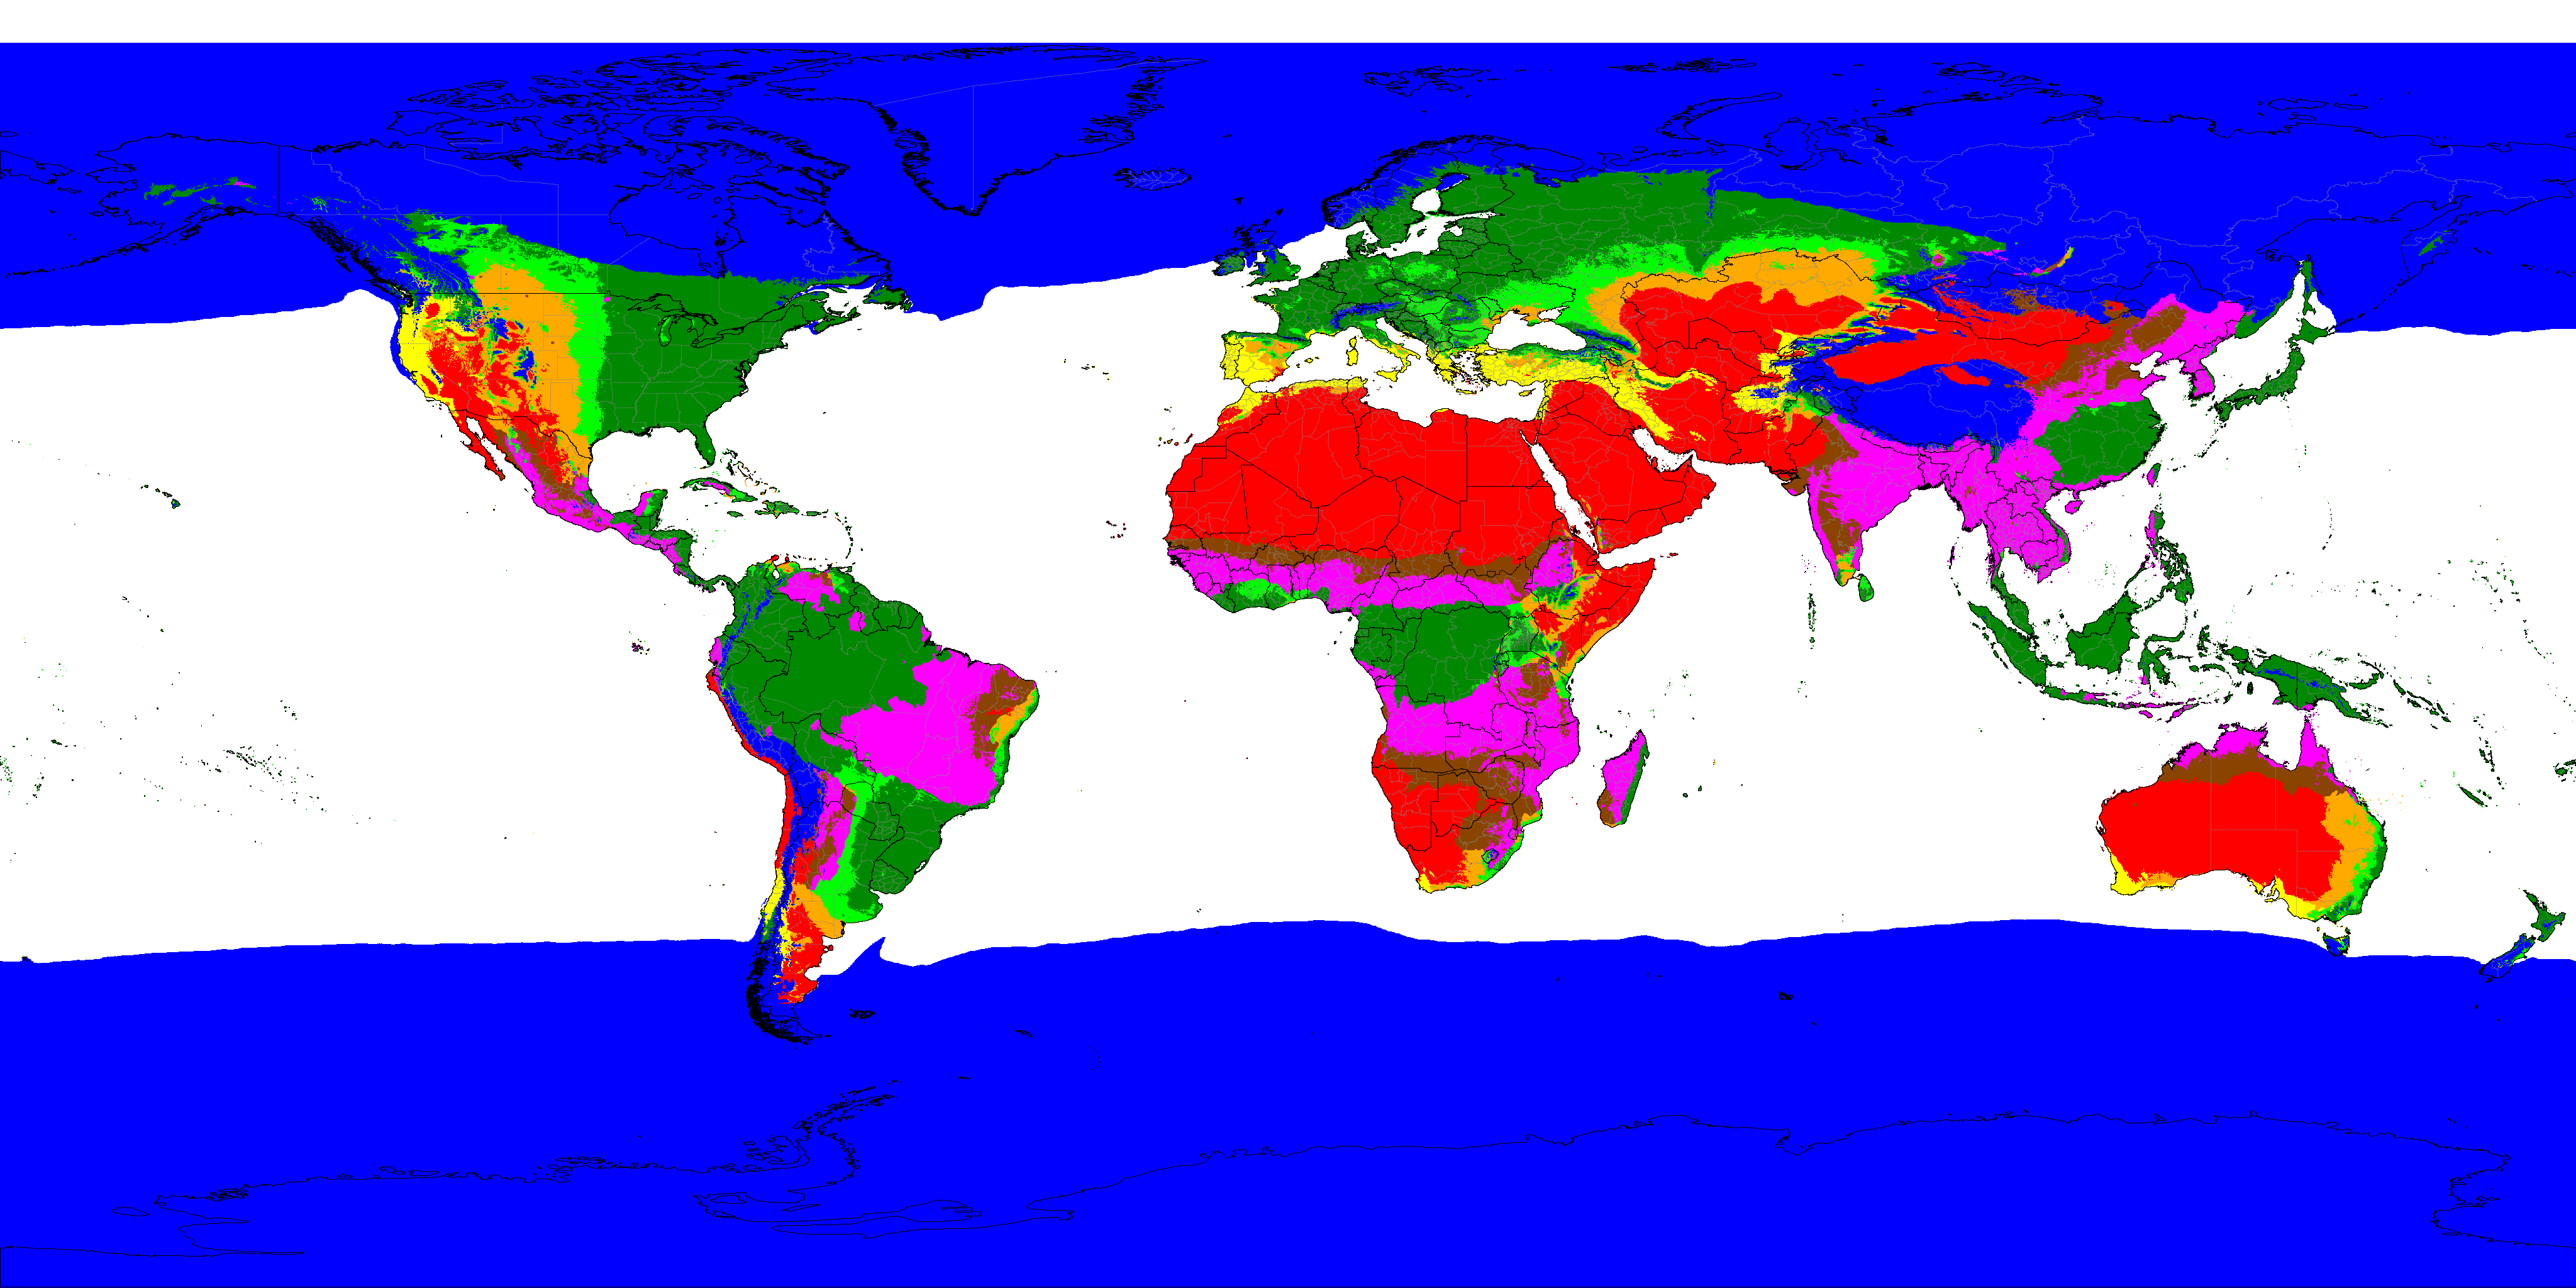
\includegraphics[width=\textwidth]{global_aridity_1981-2010.png}
\label{fig:global_aridity}
\end{figure}
\FloatBarrier

\begin{figure}[htbp]
\centering
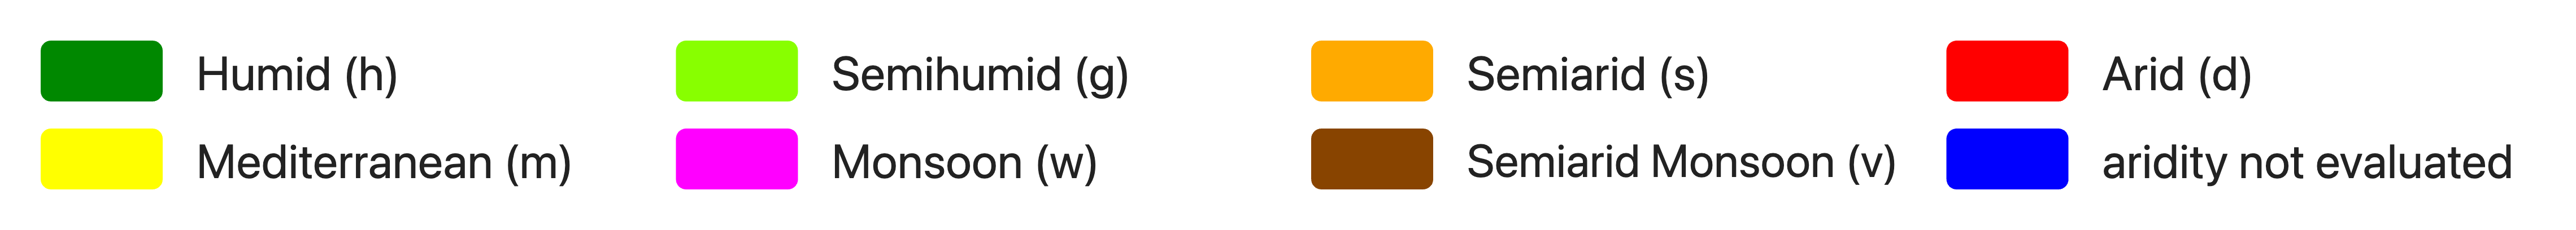
\includegraphics[width=\textwidth]{aridity_legend.png}
\caption{
Global distribution of aridity zones under the
Dickinson Climate Classification, based on 1981--2010 climatological normals.
Data were processed and plotted in Google Earth Engine (GEE) using
CHELSA BIOCLIM+ v2.1 1981--2010 precipitation and Penman-Monteith PET fields (Allen et al., 1998; Karger et al., 2017; Brun et al., 2022).
}
\label{fig:aridity_legend}
\end{figure}

\clearpage

% ============================================================
\section{Illustrative Climate Codes}

The following examples demonstrate the semantic interpretation of
Dickinson climate codes.  
Each code is composed of a cold-month thermal zone, an aridity regime
(where applicable), and a warm-month thermal zone, as defined in the
preceding sections.  
These examples are illustrative only and do not necessarily exist on Earth.

\begin{itemize}
  \item \textbf{YY} —
  Superarctic with frigid summer.

  \item \textbf{Fa2} —
  Subarctic with hot summer.
  
  \item \textbf{Ema1} —
  Continental Mediterranean with warm summer.

  \item \textbf{CdX} —
  Subtropical arid with hyperthermal summer.
  
  \item \textbf{Bb1} —
  Tropical with cold summer.

  \item \textbf{Bhb2} —
  Tropical humid with cool summer.

  \item \textbf{Zgz2} —
  Hyperequatorial semihumid with scorching summer.

\end{itemize}

% ============================================================
\section*{Conclusion}

The Dickinson Climate Classification provides a thermodynamic partition of climate space without imposing biological assumptions or temporal constraints. By formalizing aridity relevance, seasonality diagnostics, and exception handling, the system remains stable under extreme warming, deep-time climates, and hypothetical planetary environments within the thermodynamic domain compatible with life.

% ============================================================

\section*{References}

Allen, R. G., Pereira, L. S., Raes, D., & Smith, M. (1998).
Crop evapotranspiration—Guidelines for computing crop water requirements.
FAO Irrigation and Drainage Paper No. 56. Rome: Food and Agriculture Organization of the United Nations.

Brun, P., Zimmermann, N. E., Hari, C., Pellissier, L., \& Karger, D. N. (2022).
Global climate-related predictors at kilometre resolution for the past and future.
\textit{Earth System Science Data}, 14, 5573--5603.
\url{https://doi.org/10.5194/essd-14-5573-2022}

Carpenter, E. J., Lin, S., \& Capone, D. G. (2000).
Bacterial activity in South Pole snow.
\textit{Applied and Environmental Microbiology}, 66(10), 4514--4517.
\url{https://doi.org/10.1128/AEM.66.10.4514-4517.2000}

Emanuel, K. A. (1988).
The maximum intensity of hurricanes.
\textit{Journal of the Atmospheric Sciences}, 45(7), 1143--1155.
\url{https://doi.org/10.1175/1520-0469(1988)045<1143:TMIOH>2.0.CO;2}

Holdridge, L. R. (1947).
Determination of world plant formations from simple climatic data.
\textit{Science}, 105(2727), 367--368.
\url{https://doi.org/10.1126/science.105.2727.367}

Karger, D. N., Conrad, O., Böhner, J., Kawohl, T., Kreft, H., Soria-Auza, R. W.,
Zimmermann, N. E., Linder, P., \& Kessler, M. (2017).
Climatologies at high resolution for the Earth's land surface areas.
\textit{Scientific Data}, 4, 170122.
\url{https://doi.org/10.1038/sdata.2017.122}

Köppen, W. (1884).
Die Wärmezonen der Erde, nach der Dauer der heissen, gemässigten und kalten Zeit
und nach der Wirkung der Wärme auf die organische Welt betrachtet.
\textit{Meteorologische Zeitschrift}, 1, 215--226.

United Nations Environment Programme. (1992).
\textit{World Atlas of Desertification} (2nd ed.).
Edward Arnold.

\end{document}
